\documentclass{beamer}
\usepackage[utf8]{inputenc}

\usepackage{color}
\usepackage{xcolor}
%\definecolor{PLB}{rgb}{0.06,0.42,0.60}
%\definecolor{PLBfonce}{rgb}{0.06,0.42,0.60}
%\definecolor{PLBmoyen}{RGB}{176, 216, 232}
%\definecolor{PLBpale}{rgb}{0.94,0.965,0.965}

%\definecolor{PLB}{HTML}{424242}
\definecolor{PLB}{HTML}{1289A7}
\definecolor{PLBfonce}{rgb}{0.06,0.42,0.60}
\definecolor{PLBmoyen}{RGB}{176, 216, 232}
\definecolor{PLBpale}{rgb}{0.94,0.965,0.965}

%\usetheme{PaloAlto}
\usetheme{Madrid}
\setbeamercolor{frametitle}{bg=PLB}     %controls the color of the headline
\setbeamercolor{sidebar}{bg=PLB}        %controls the color of the sidebar
\setbeamercolor{logo}{bg=PLB!70!black}
\setbeamercolor{structure}{fg=PLB, bg=PLB!40}
%\setbeamertemplate{footline}[default]
\setbeamertemplate{footline}[frame number]{}
\setbeamertemplate{enumerate items}[square]
\setbeamertemplate{itemize items}[circle]

\setbeamerfont{section number projected}{size=\large}
\setbeamertemplate{section in toc}[circle]
\setbeamertemplate{subsection in toc}[square]

\usepackage{amssymb}
\usepackage{pifont}
\usepackage{bigints}
\usepackage{mathrsfs}
\usepackage{physics}

\definecolor{mblue}{rgb}{0.18,0.21,0.67}
\definecolor{mgree}{rgb}{0.,0.6,0.}
\definecolor{mred}{HTML}{EA2027}
\definecolor{dgreen}{HTML}{009432}
\definecolor{morange}{HTML}{F79F1F}
\definecolor{violet}{HTML}{9980FA}
\definecolor{bleu}{RGB}{41, 128, 185}
\definecolor{gris}{rgb}{0.5,0.5,0.5}
\definecolor{fluid}{HTML}{6ab04c}
\definecolor{kinetic}{HTML}{f0932b}
\newcommand{\cmark}{{\color{dgreen}\ding{52}}}
\newcommand{\xmark}{{\color{mred}\ding{55}}}
\newcommand{\bmark}{{\color{morange}$\sim$}}
\newcommand{\arrow}{{\color{PLB}\ding{220}}}
\newcommand{\mbold}[1]{{\textbf{\color{PLB}#1}}}

\usepackage{soul}
\usepackage{multicol}
\usepackage{multirow}

\usepackage{rotating}

\usepackage{ifthen}

\usepackage{amsmath}
\usepackage{cancel}
\DeclareMathOperator*{\argmax}{argmax}
\DeclareMathOperator*{\argmin}{argmin}
\DeclareMathOperator\erfi{erfi}

\usepackage[backend=bibtex, style=authoryear-comp]{biblatex}
\usepackage{filecontents}
\renewbibmacro*{cite}{%
  \begin{footnotesize}
  \iffieldundef{shorthand}
    {\ifthenelse{\ifnameundef{labelname}\OR\iffieldundef{labelyear}}
       {\usebibmacro{cite:label}%
        \setunit{\printdelim{nonameyeardelim}}}
       {\printnames{labelname}%
        \setunit{\printdelim{nameyeardelim}}}%
     \usebibmacro{cite:labeldate+extradate}%
     \setunit{\addcomma\space}%
     \usebibmacro{journal}}
    {\usebibmacro{cite:shorthand}}\end{footnotesize}}
%\newcommand{\customcite}[1]{\citeauthor{#1} (\citeyear{#1})}
\newcommand{\customcite}[1]{\cite{#1}}

\bibliography{biblio}

\beamertemplatenavigationsymbolsempty

\usepackage{bm}
\newcommand{\Mvb}[1]{\boldsymbol{#1}}
\newcommand{\I}{\dot{\imath}}

%for backup slides
\newcommand{\backupbegin}{
  \newcounter{finalframe}
  \setcounter{finalframe}{\value{framenumber}}
}
\newcommand{\backupend}{
  \setcounter{framenumber}{\value{finalframe}}
}


\AtBeginSection[
  {\frame<beamer>{\frametitle{Outline}   
    \tableofcontents[currentsection,currentsection]}}%
]%
{
  \frame<beamer>{ 
    \frametitle{Outline}   
    \tableofcontents[currentsection,currentsection]}
}

\newenvironment{bframe}[1]% frame of backup (to get bakcup in title) 
{% begin code
  \begin{frame}{{\small\texttt{backup}\ } #1}
}%
{% end code
  \end{frame}
}

\newcommand{\colorsec}{\color{PLB}}

\newcommand{\changecolor}[1]{%
  %\begingroup

  \setbeamercolor{frametitle}{bg=#1}
  \setbeamercolor{sidebar}{bg=#1}
  \setbeamercolor{logo}{bg=#1!70!black}
  \setbeamercolor{structure}{fg=#1, bg=#1!40}

  \renewcommand{\arrow}{{\color{#1}\ding{220}}}
  \renewcommand{\mbold}[1]{{\textbf{\color{#1}##1}}}

  %\endgroup
}

\definecolor{sec1}{HTML}{1289A7} %{F79F1F}
\definecolor{sec2}{HTML}{1289A7} %{A3CB38}
\definecolor{sec3}{HTML}{1289A7}
\definecolor{sec4}{HTML}{1289A7} %{D980FA}
\definecolor{sec5}{HTML}{1289A7} %{B53471}

%\title[Workshop Bordeaux]{Hybrid model of Vlasov-Maxwell equations\\ and\\ comparison of Hamiltonian method and Lawson method}
\title[]{Méthodes numériques pour des modèles hybrides fluide-cinétique de plasmas}
\author[]{Josselin Massot}
\date[]{16 décembre 2021}

\AtBeginDocument{\colorlet{defaultcolor}{.}}

\begin{document}
% -------------------------------------------------------------------
% --- BEGIN DOCUMENT ------------------------------------------------
% -------------------------------------------------------------------

\begin{frame}[plain]
  \titlepage
  \begin{tabular}{lrl}
    Directeur de thèse :     & Nicolas & Crouseilles \\
    Co-Directrice de thèse : & Anaïs   & Crestetto \\
  \end{tabular}
\end{frame}
\begin{frame}{Outline}
  \tableofcontents
\end{frame}

% -------------------------------------------------------------------
% --- INTRODUCTION --------------------------------------------------
% -------------------------------------------------------------------
\changecolor{sec1}
\section{Introduction}
\begin{frame}{Vlasov-Maxwell $1dz-3dv$ model}
  Transport of electron density distribution $f=f(t,z,\Mvb{v})$,\\
  $\Mvb{B}(t,z)=(B_x,B_y,0)(t,z),\Mvb{E}(t,z)=(E_x,E_y,0)(t,z)\in\mathbb{R}^2$,\\
  $z\in[0,2\pi]$, $\Mvb{B}_0 = (0,0,B_0)^\top$, $\Mvb{v}\in\mathbb{R}^3$, $v_\perp=(v_x,v_y)^\top\in\mathbb{R}^2$:

  $$
    \begin{cases}
      \partial_t f + v_z\partial_z f - (\Mvb{E}+\Mvb{v}\times(\Mvb{B}+\Mvb{B}_0))\cdot\nabla_{\Mvb{v}} f = 0 \\
      \partial_t \Mvb{B} = -\partial_z\Mvb{E}\\
      \partial_t \Mvb{E} = \partial_z\Mvb{B} + \int_{\mathbb{R}^3} v_\perp f\dd{\Mvb{v}} \\
    \end{cases}
  $$
  \begin{figure}
    \centering
    \vspace{-1cm}
    \hspace{5cm}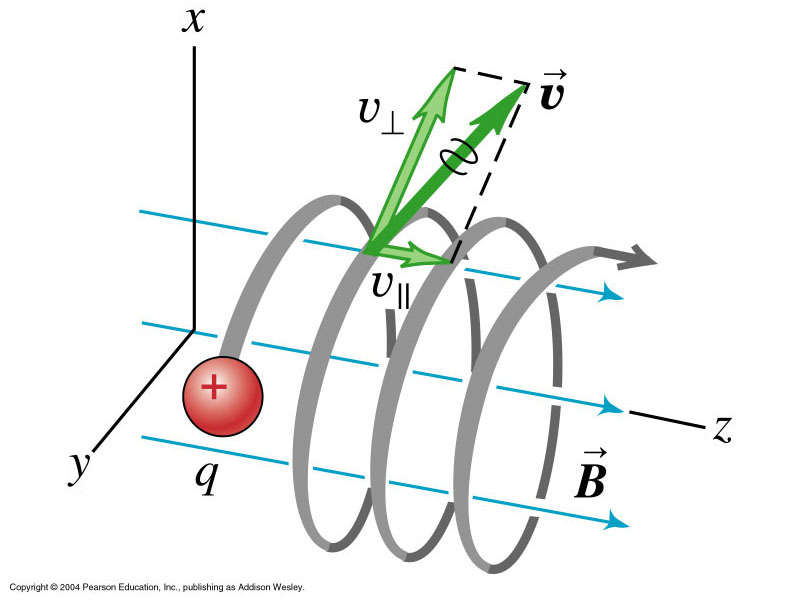
\includegraphics[height=0.5\textheight]{img/helix}
  \end{figure}
\end{frame}
\begin{frame}{Vlasov-Maxwell $1dz-3dv$ model}{Motivation:}
\begin{itemize}
  \item We want high order methods in $(z,\Mvb{v})$ \begin{itemize}\item FFT in $z$ + WENO in $\Mvb{v}$\end{itemize}
  \item We want high order methods in time $t$ \begin{itemize}\item splitting method vs exponential integrator\end{itemize}
\end{itemize}
\begin{figure}
  \centering
  % GNUPLOT: LaTeX picture with Postscript
\begingroup
\newcommand{\ft}[0]{\footnotesize}
  \makeatletter
  \providecommand\color[2][]{%
    \GenericError{(gnuplot) \space\space\space\@spaces}{%
      Package color not loaded in conjunction with
      terminal option `colourtext'%
    }{See the gnuplot documentation for explanation.%
    }{Either use 'blacktext' in gnuplot or load the package
      color.sty in LaTeX.}%
    \renewcommand\color[2][]{}%
  }%
  \providecommand\includegraphics[2][]{%
    \GenericError{(gnuplot) \space\space\space\@spaces}{%
      Package graphicx or graphics not loaded%
    }{See the gnuplot documentation for explanation.%
    }{The gnuplot epslatex terminal needs graphicx.sty or graphics.sty.}%
    \renewcommand\includegraphics[2][]{}%
  }%
  \providecommand\rotatebox[2]{#2}%
  \@ifundefined{ifGPcolor}{%
    \newif\ifGPcolor
    \GPcolortrue
  }{}%
  \@ifundefined{ifGPblacktext}{%
    \newif\ifGPblacktext
    \GPblacktexttrue
  }{}%
  % define a \g@addto@macro without @ in the name:
  \let\gplgaddtomacro\g@addto@macro
  % define empty templates for all commands taking text:
  \gdef\gplbacktext{}%
  \gdef\gplfronttext{}%
  \makeatother
  \ifGPblacktext
    % no textcolor at all
    \def\colorrgb#1{}%
    \def\colorgray#1{}%
  \else
    % gray or color?
    \ifGPcolor
      \def\colorrgb#1{\color[rgb]{#1}}%
      \def\colorgray#1{\color[gray]{#1}}%
      \expandafter\def\csname LTw\endcsname{\color{white}}%
      \expandafter\def\csname LTb\endcsname{\color{black}}%
      \expandafter\def\csname LTa\endcsname{\color{black}}%
      \expandafter\def\csname LT0\endcsname{\color[rgb]{1,0,0}}%
      \expandafter\def\csname LT1\endcsname{\color[rgb]{0,1,0}}%
      \expandafter\def\csname LT2\endcsname{\color[rgb]{0,0,1}}%
      \expandafter\def\csname LT3\endcsname{\color[rgb]{1,0,1}}%
      \expandafter\def\csname LT4\endcsname{\color[rgb]{0,1,1}}%
      \expandafter\def\csname LT5\endcsname{\color[rgb]{1,1,0}}%
      \expandafter\def\csname LT6\endcsname{\color[rgb]{0,0,0}}%
      \expandafter\def\csname LT7\endcsname{\color[rgb]{1,0.3,0}}%
      \expandafter\def\csname LT8\endcsname{\color[rgb]{0.5,0.5,0.5}}%
    \else
      % gray
      \def\colorrgb#1{\color{black}}%
      \def\colorgray#1{\color[gray]{#1}}%
      \expandafter\def\csname LTw\endcsname{\color{white}}%
      \expandafter\def\csname LTb\endcsname{\color{black}}%
      \expandafter\def\csname LTa\endcsname{\color{black}}%
      \expandafter\def\csname LT0\endcsname{\color{black}}%
      \expandafter\def\csname LT1\endcsname{\color{black}}%
      \expandafter\def\csname LT2\endcsname{\color{black}}%
      \expandafter\def\csname LT3\endcsname{\color{black}}%
      \expandafter\def\csname LT4\endcsname{\color{black}}%
      \expandafter\def\csname LT5\endcsname{\color{black}}%
      \expandafter\def\csname LT6\endcsname{\color{black}}%
      \expandafter\def\csname LT7\endcsname{\color{black}}%
      \expandafter\def\csname LT8\endcsname{\color{black}}%
    \fi
  \fi
    \setlength{\unitlength}{0.0500bp}%
    \ifx\gptboxheight\undefined%
      \newlength{\gptboxheight}%
      \newlength{\gptboxwidth}%
      \newsavebox{\gptboxtext}%
    \fi%
    \setlength{\fboxrule}{0.5pt}%
    \setlength{\fboxsep}{1pt}%
    \definecolor{tbcol}{rgb}{1,1,1}%
\begin{picture}(8100.00,2268.00)%
    \gplgaddtomacro\gplbacktext{%
      \csname LTb\endcsname%%
      \put(330,536){\makebox(0,0)[r]{\strut{}$0$}}%
      \put(330,1080){\makebox(0,0)[r]{\strut{}$0.25$}}%
      \put(330,1624){\makebox(0,0)[r]{\strut{}$0.5$}}%
      \put(330,2168){\makebox(0,0)[r]{\strut{}$0.75$}}%
      \put(390,273){\makebox(0,0){\strut{}$-10$}}%
      \put(2272,273){\makebox(0,0){\strut{}$-5$}}%
      \put(4154,273){\makebox(0,0){\strut{}$0$}}%
      \put(6036,273){\makebox(0,0){\strut{}$5$}}%
      \put(7918,273){\makebox(0,0){\strut{}$10$}}%
    }%
    \gplgaddtomacro\gplfronttext{%
      \csname LTb\endcsname%%
      \put(4154,70){\makebox(0,0){\strut{}$v$}}%
      \csname LTb\endcsname%%
      \put(3966,1320){\makebox(0,0)[l]{\strut{}\ft $\sqrt{T_c}$}}%
      \put(2046,840){\makebox(0,0)[l]{\strut{}$-v_0$}}%
      \put(5923,840){\makebox(0,0)[l]{\strut{}$v_0$}}%
    }%
    \gplbacktext
    \put(0,0){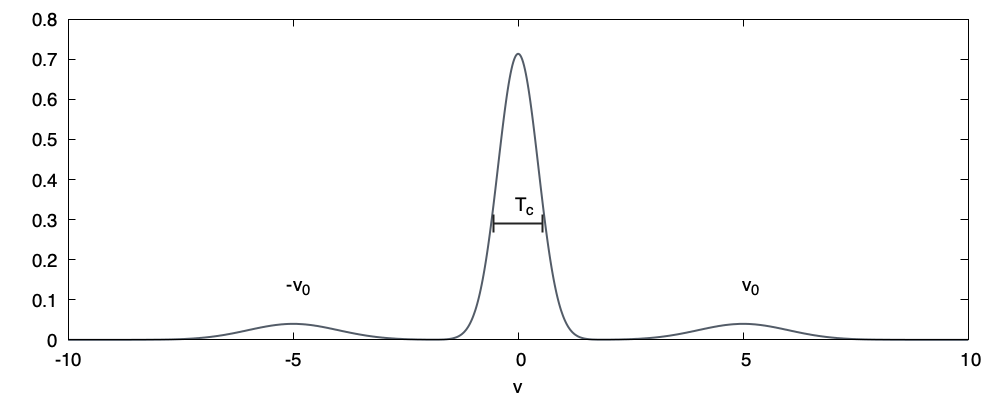
\includegraphics[width={405.00bp},height={113.40bp}]{./intro/figures/distrib}}%
    \gplfronttext
  \end{picture}%
\endgroup

\end{figure}
\begin{itemize}
  \item We consider an initial condition of the form $f = \textcolor{fluid}{f_c}+\textcolor{kinetic}{f_h}$ with: $\textcolor{fluid}{f_c(t=0,z,\Mvb{v})}=\textcolor{fluid}{\rho_c(t,z)}\delta_{\Mvb{v}=\textcolor{fluid}{\Mvb{u}_c(t,z)}}(\Mvb{v})$
\end{itemize}
\end{frame}
\begin{frame}{The idea}
  Grid methods can't have an initial condition like:
  $$
    f_0(z,\Mvb{v}) = \underbrace{\rho_{c,0}(z)\textcolor{mred}{\delta_{\Mvb{v}-\Mvb{u}_c}(\Mvb{v})}}_{\textcolor{fluid}{f_{c,0}}} + \textcolor{kinetic}{f_{h,0}(z,\Mvb{v})}
  $$
  The main idea is to derive an \mbold{linearized hybrid \textcolor{fluid}{fluid}/\textcolor{kinetic}{kinetic} model}:
    \begin{itemize}
      \item Split $f=\textcolor{fluid}{f_c}+\textcolor{kinetic}{f_h}$ (2 Vlasov equations)
      \item Compute momentum of $\textcolor{fluid}{f_c}$
        \begin{itemize}
          \item \emph{Cold plasma approximation}: $\frac{T_c}{T_h}\ll 1$\arrow $\cancel{\textcolor{fluid}{f_c(t,z,\Mvb{v})}}$ \arrow $\textcolor{fluid}{\Mvb{j}_c(t,z)}$
          \item Fluid dynamic for cold particles (no velocity grid) \cmark{}
          \item Linearized fluid equations
        \end{itemize}
      \item Hypothesis on hot particles: $\int_{\mathbb{R}^3} \textcolor{kinetic}{f_h(t,z,\Mvb{v})}\dd{\Mvb{v}} \ll \textcolor{fluid}{\rho_c(t,z)}$
        \begin{itemize}
          \item Kinetic dynamic for hot particles
        \end{itemize}
    \end{itemize}

  \vfill
 
  \begin{thebibliography}{9}
    \setbeamertemplate{bibliography item}[article]
    \bibitem{b} \customcite{Tronci:2014}
    \vspace{-0.25cm}
    \bibitem{a} \customcite{Holderied:2020}
  \end{thebibliography}
\end{frame}

\begin{frame}{Linearized hybrid Vlasov-Maxwell $1dz-3dv$ model}
  The new model: a nonlinear transport in $(z,v_x,v_y,v_z)\in\Omega\times\mathbb{R}^3$ of:
  \begin{itemize}
    \item a cold (\textcolor{fluid}{fluid}) electron density distribution, reconstruction from current variable $\textcolor{fluid}{\Mvb{j}_c(t,z)} = q_e\textcolor{fluid}{\rho_c(t,z)}\textcolor{fluid}{\Mvb{u}_c(t,z)}
    =(\textcolor{fluid}{j_{c,x}},\textcolor{fluid}{j_{c,y}},0)(t,z)$
    \item a hot (\textcolor{kinetic}{kinetic}) electron density distribution $\textcolor{kinetic}{f_h(t,z,\Mvb{v})}$
  \end{itemize}
  $$
    \begin{cases}
      \textcolor{fluid}{\partial_t\Mvb{j}_c = \Omega_{pe}^2\Mvb{E} - J\Mvb{j}_c B_0} \\
      \partial_t\Mvb{B}   = J\partial_z\Mvb{E} \\
      \partial_t\Mvb{E}   = -J\partial_z\Mvb{B} - \textcolor{fluid}{\Mvb{j}_c} + \int_{\mathbb{R}^3} v_\perp \textcolor{kinetic}{f_h}\dd{\Mvb{v}} \\
      \textcolor{kinetic}{\partial_t f_h  + v_z\partial_z f_h - \left( \Mvb{E} + \Mvb{v}\times(\Mvb{B}+\Mvb{B}_0) \right)\cdot\nabla_{\Mvb{v}} f_h = 0}
    \end{cases}
  $$
  with:
  $$
    J = \begin{pmatrix}
       0 & 1 \\
      -1 & 0
    \end{pmatrix}
  $$
  %we define the Hamiltonian as :
  %$$
  %  \begin{aligned}
  %    \mathcal{H} &=
  %      \underbrace{\frac{1}{2}\int \|\Mvb{E}\|^2 \dd{z}}_{\mathcal{H}_E}
  %    + \underbrace{\frac{1}{2}\int \|\Mvb{B}\|^2 \dd{z}}_{\mathcal{H}_B}
  %    + \underbrace{\frac{1}{2}\int \frac{1}{\Omega_{pe}^2}\|\Mvb{j}_c\|^2 \dd{z}}_{\mathcal{H}_{j_c}}\\
  %    &\qquad+ \underbrace{\frac{1}{2}\int\int \|\Mvb{v}\|^2f_h \dd{\Mvb{v}}\dd{z}}_{\mathcal{H}_{f_h}}
  %  \end{aligned}
  %$$
\end{frame}

\begin{frame}{Convergence when $T_c\to 0$ for 1dx-1dv model}
  \begin{figure}
    \centering
    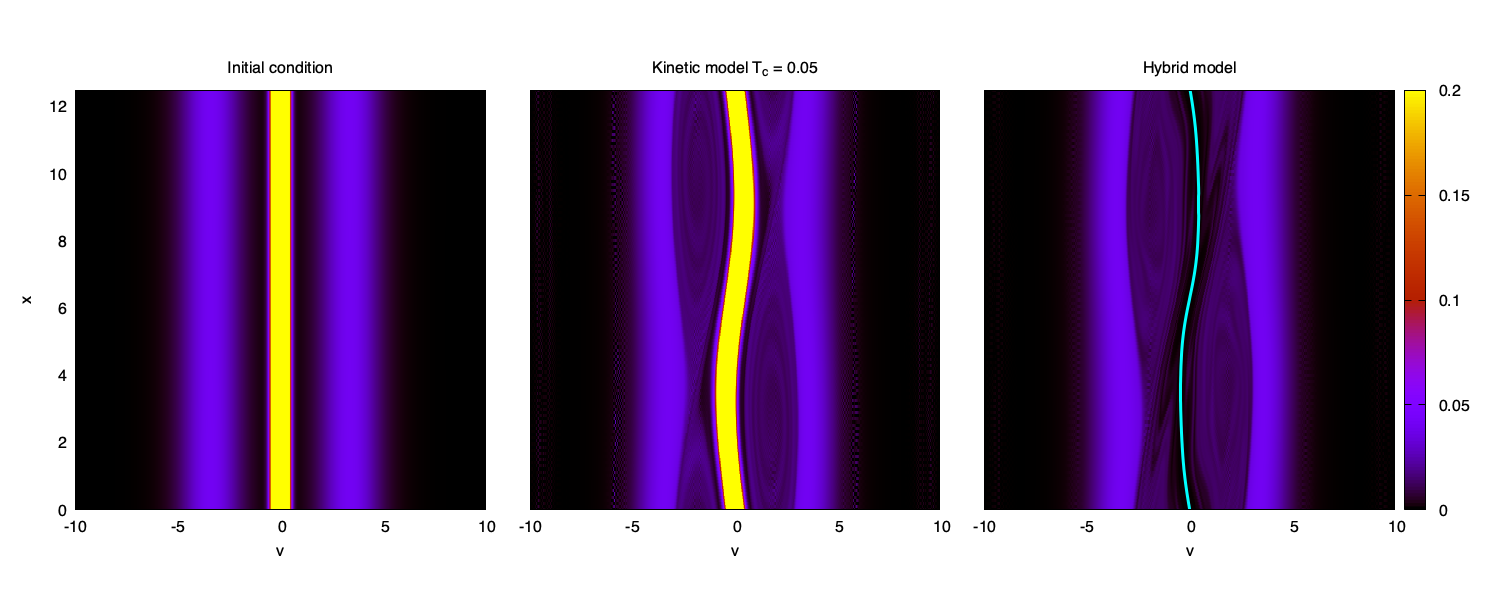
\includegraphics[width=\textwidth]{img/vp_t1}
    \caption{Simulation of initial condition (left) with kinetic model with $T_c=0.05$ (middle) and hybrid model (right) to the time $T_f=200$}
  \end{figure}
  \cmark{} Good agreement between kinetic ($f$) model and hybrid model ($\textcolor{kinetic}{f_h}$ \mbold{+} $\textcolor{fluid}{u_c}$)
\end{frame}


% -------------------------------------------------------------------
% --- NUMERICAL METHODS ---------------------------------------------
% -------------------------------------------------------------------
\changecolor{sec2}
\section{Numerical methods}
\begin{frame}{Numerical methods}
  Two time integrators to compute a numerical solution of abstract model:
  $$
    \dot{u} = L(t,u) + N(t,u),\quad u(0) = u_0
  $$
  $u\in\mathbb{R}^d$, $L$ and $N$ functions $(t,u)\in\mathbb{R}_+\times\mathbb{R}^d\mapsto\mathbb{R}^d$, $d\in\mathbb{N}$.
  \vfill
  \begin{itemize}
    \item Splitting method (Lie, Strang, Suzuki)
    \item Lawson method (LRK(4,4), LDP4(3))
  \end{itemize}
  \vfill
  
  In space $z$: we use a Fourier transform (FFT).

  In velocity $\Mvb{v}$: we use WENO5 or Lagrange 5.
\end{frame}
\begin{frame}{Splitting method}
  Successive resolution of:
  $$
    \begin{aligned}
      \dot{u} &= Lu     \qquad & \rightarrow \tilde{u}_t = \varphi^{[L]}_t(u_0) \\
      \dot{u} &= N(t,u)        & \rightarrow \tilde{u}_t = \varphi^{[N]}_t(u_0)
    \end{aligned}
  $$
  Solution at time $t$:
  \begin{description}
    \item[\mbold{Lie:}] order 1 method, composition of sub-steps:
        $\varphi_t(u_0) \approx \varphi_t^{[L]} \circ \varphi_t^{[N]}(u_0)$
    \item[\mbold{Strang:}] order 2 method:
        $\varphi_t(u_0) \approx \mathcal{S}_t(u_0) = \varphi_{t/2}^{[L]} \circ \varphi_t^{[N]} \circ \varphi_{t/2}^{[L]} (u_0)$
        \vspace{-0.25cm}
        \begin{thebibliography}{9}
          \setbeamertemplate{bibliography item}[article]
          \bibitem{b} \customcite{Strang:1968}
        \end{thebibliography}
    \item[\mbold{Suzuki:}] order 4 method, composition of 5 Strang methods:
        $$\varphi_t(u_0) \approx \mathcal{S}_{\alpha_1t}\circ\mathcal{S}_{\alpha_2t}\circ\mathcal{S}_{\alpha_3t}\circ\mathcal{S}_{\alpha_2t}\circ\mathcal{S}_{\alpha_1t}(u_0)$$
        with:
        $\alpha_1 = \alpha_2 = \frac{1}{4-\sqrt[3]{4}}$ and $\alpha_3 = \frac{1}{1-4^{\frac{2}{3}}}$
        \vspace{-0.25cm}
        \begin{thebibliography}{9}
          \setbeamertemplate{bibliography item}[article]
          \bibitem{c} \customcite{Suzuki:1990}
        \end{thebibliography}
  \end{description}
\end{frame}
%-------%
\begin{frame}{Splitting method}
  {Pros \& Cons}
  \begin{description}
    \item[\cmark] Good splitting leads to good long time behavior
    \item[\cmark] Error in time only depends on splitting method
    \item[\cmark] Split a difficult problem into small easier sub-problems
    \item[\xmark] Numerical cost for high order method
  \end{description}
  
\end{frame}

%-------%
\begin{frame}{Lawson method}
  $$
    \partial_t u = Lu + N(t,u)
  $$
  Change of variable: \mbold{$v = e^{-tL}u$}, we obtain:
  $$
    \begin{aligned}
      \dot{v}(t) &= -Le^{-tL}u(t) + e^{-tL}\underbrace{\left(Lu(t) + N(t,u)\right)}_{\dot{u}(t)} \\
                 &= e^{-tL}N(t,e^{tL}v)
    \end{aligned}
  $$
  which can be solved with a \mbold{Runge-Kutta method} in $v$, that can be rewritten in $u$, for example with Euler method:
  $$
    v(t^n+\Delta t) \approx v^{n+1} = v^n + \Delta t e^{-t^nL}N(t^n,e^{t^nL}v^n)
  $$
  or as an expression of $u$ :
  $$
    u^{n+1} = e^{\Delta t L}u^n + \Delta te^{\Delta t L}N(t^n,u^n)
  $$
  \begin{thebibliography}{9}
    \setbeamertemplate{bibliography item}[article]
    \bibitem{e} \customcite{Lawson:1967a} \vspace{-0.25cm}
    \bibitem{f} \customcite{Hochbruck:2010} \vspace{-0.25cm}
    \bibitem{g} \customcite{Hochbruck:2020}
  \end{thebibliography}
\end{frame}
%-------%
\begin{frame}{Lawson method}
  {Pros \& Cons}
  \begin{description}
    \item[\cmark] Numerically efficient (order increases linearly-ish with the number of stages)
    \item[\cmark] Literature on Runge-Kutta method (embedded-RK, low storage methods, IMEX methods, DIRK methods\dots)
    \item[\cmark] Linear part is solved exactly
    \item[\xmark] Stability constraint (not from the linear part \cmark)
    \item[\xmark] Behavior in long time
    \item[\bmark] Needs to compute (efficiently) $e^{\tau L}$ for any $\tau=c_j\Delta t$ and $L$
  \end{description}
\end{frame}

%-------%
\begin{frame}{Main idea of adaptive time step methods (error estimate)}
  For a generic ODE $\dot{u} = f(t,u)$, adaptive time step method needs 2 numerical estimations of solution $u(t^{n+1})$ of different order, $p$ and $p+1$:
  $$
    u^{n+1}_{[p]} = u(t^{n+1}) + \order{\Delta t^{p+1}},\qquad u^{n+1}_{[p+1]} = u(t^{n+1}) + \order{\Delta t^{p+2}}
  $$
  Estimate of local error:
  \vspace{-0.5cm}
  $$
    L_{[p]}^{n+1} = \left| u^{n+1}_{[p+1]} - u^{n+1}_{[p]} \right|
  $$
  \mbold{If $L^{n+1}_{[p]}>tol$:} we reject the step and start again from time $t^n$. \mbold{Else} we accept the step. \mbold{In both cases}, the optimal new time step is:
  $$
    \Delta t_\text{opt} = \sqrt[p]{\frac{tol}{L^{n+1}_{[p]}}}\Delta t^n
  $$
  In practice $u^{n+1}_{[p]}$ is computed from sub-steps of $u^{n+1}_{[p+1]}$.

  \begin{thebibliography}{9}
    \setbeamertemplate{bibliography item}[article]
    \bibitem{g} \customcite{Dormand:1978} \textcolor{defaultcolor}{(for RK method)}
    \bibitem{h} \customcite{Blanes:2019} \textcolor{defaultcolor}{(for splitting method)}
  \end{thebibliography}
  %In practice we don't want volatile time step:
  %$
  %  \Delta t^{n+1} = \max\left( 0.5\Delta t^n , \min\left( 2\Delta t^n , \Delta t_\text{opt} \right) \right)
  %$
\end{frame}

% -------------------------------------------------------------------
% --- APPLICATION FOR HYBRID VLASOV-MAXWELL MODEL -------------------
% -------------------------------------------------------------------
\changecolor{sec3}
\section{Application for hybrid Vlasov-Maxwell model}
\begin{frame}{Linearized hybrid Vlasov-Maxwell model}
  $U = \left(\textcolor{fluid}{\Mvb{j}_c} , \Mvb{B} , \Mvb{E} , \textcolor{kinetic}{f_h} \right)^\top$, $\textcolor{fluid}{\Mvb{j}_c}(t,z)$,$\Mvb{B}(t,z)$,$\Mvb{E}(t,z)\in\mathbb{R}^2$,$\textcolor{kinetic}{f_h}(t,z,\Mvb{v})\in\mathbb{R}$
  $$
    \begin{cases}
      \partial_t\textcolor{fluid}{\Mvb{j}_c} = \Omega_{pe}^2\Mvb{E} - J\textcolor{fluid}{\Mvb{j}_c} B_0 \\
      \partial_t\Mvb{B}   = J\partial_z\Mvb{E} \\
      \partial_t\Mvb{E}   = -J\partial_z\Mvb{B} - \textcolor{fluid}{\Mvb{j}_c} + \int v_\perp \textcolor{kinetic}{f_h}\dd{v_\perp} \\
      \partial_t \textcolor{kinetic}{f_h}  + v_z\partial_z \textcolor{kinetic}{f_h} - \left( \Mvb{E} + \Mvb{v}\times(\Mvb{B}+\Mvb{B}_0) \right)\cdot\nabla_{\Mvb{v}} \textcolor{kinetic}{f_h} = 0
    \end{cases}
  $$
  we define the Hamiltonian as :
  $$
    \begin{aligned}
      \mathcal{H} &=
        \underbrace{\frac{1}{2}\int \|\Mvb{E}\|^2 \dd{z}}_{\mathcal{H}_E}
      + \underbrace{\frac{1}{2}\int \|\Mvb{B}\|^2 \dd{z}}_{\mathcal{H}_B}
      + \underbrace{\frac{1}{2}\int \frac{1}{\Omega_{pe}^2}\|\textcolor{fluid}{\Mvb{j}_c}\|^2 \dd{z}}_{\mathcal{H}_{j_c}}\\
      &\qquad+ \underbrace{\frac{1}{2}\int\int \|\Mvb{v}\|^2\textcolor{kinetic}{f_h} \dd{\Mvb{v}}\dd{z}}_{\mathcal{H}_{f_h}}
    \end{aligned}
  $$
  Following the Hamiltonian we built a Hamiltonian splitting.
\end{frame}
%-------%
\subsection{With splitting method}
\begin{frame}{Splitting method}
  5 subsystems $\varphi^{[E]}$, $\varphi^{[B]}$, $\varphi^{[j_c]}$, $\varphi^{[f_h]}$


  \begin{itemize}
    \item Solution with Lie splitting method:
      $$
        U^{n+1} = \varphi_{\Delta t}^{[E]}
            \circ \varphi_{\Delta t}^{[B]}
            \circ \varphi_{\Delta t}^{[j_c]}
            \circ \varphi_{\Delta t}^{[f_h]} (U^n)
      $$
    \item or Strang method:
      $$
        U^{n+1} = \varphi_{\Delta t/2}^{[E]}
            \circ \varphi_{\Delta t/2}^{[B]}
            \circ \varphi_{\Delta t/2}^{[j_c]}
            \circ \varphi_{\Delta t}^{[f_h]}
            \circ \varphi_{\Delta t/2}^{[j_c]}
            \circ \varphi_{\Delta t/2}^{[B]}
            \circ \varphi_{\Delta t/2}^{[E]} (U^n)
      $$
  \end{itemize}

  \mbold{Numerical cost:}
  \begin{itemize}
    \item $\varphi^{[B]}$ and $\varphi^{[j_c]}$: almost free ($\mathcal{O}(N_z)$)
    \item $\varphi^{[E]}$: moderately expensive ($\mathcal{O}(N_z)$ \mbold{+} loop on phase space)
    \item $\varphi^{[f_h]}$: extremely expensive (multiple loops on phase space)
  \end{itemize}
\end{frame}
%-------%
\begin{frame}{Splitting method}{Example with: $\varphi^{[E]}$}
  One of sub-steps of Hamiltonian splitting:
  $$
    \varphi^{[E]}(U) =
    \begin{cases}
      \partial_t \Mvb{j}_c = \Omega_{pe}^2\Mvb{E} \\
      \partial_t \Mvb{B} = J\partial_z\Mvb{E} \\
      \partial_t \Mvb{E} = 0 \\
      \partial_t f_h = \Mvb{E}\cdot\nabla_{v_\perp}f_h
    \end{cases}
    \rightarrow
    \varphi_{t}^{[E]}(U^0) = \begin{pmatrix}
      \Mvb{j}_c(0) + t\Omega_{pe}^2\Mvb{E}(0) \\
      \Mvb{B}(0) + tJ\partial_z\Mvb{E}(0) \\
      \Mvb{E}(0) \\
      f_h(0,z,v_\perp\!+t\Mvb{E}(0),v_z)
    \end{pmatrix}
  $$
  \mbold{Numerical tools:}
  \begin{itemize}
    \item 2D interpolation with 2 Lagrange 5 interpolations to approximate $f_h(0,z,v_\perp+t\Mvb{E}(0),v_z)$
  \end{itemize}
\end{frame}

%-------%

\newcommand{\gz}{\textcolor{gris!50}{0}}

\subsection{With Lawson method}
\begin{frame}{Lawson method}
  $$\partial_tU = LU + N(t,U)$$
  with:
  $$
    L \!=\!\begin{pmatrix}
      \gz      & \!-\!B_0\! & \gz            &  \gz              &  \!\Omega_{pe}^2\! & \gz               & \gz \\ 
      \!B_0\!  &  \gz       & \gz            &  \gz              &  \gz               & \!\Omega_{pe}^2\! & \gz \\
      \gz      &  \gz       & \gz            &  \gz              &  \gz               & \partial_z        & \gz \\ 
      \gz      &  \gz       & \gz            &  \gz              & \!-\!\partial_z\!  & \gz               & \gz \\ 
      \!-\!1\! &  \gz       & \gz            & \!-\!\partial_z\! &  \gz               & \gz               & \gz \\ 
      \gz      & \!-\!1\!   & \!\partial_z\! &  \gz              &  \gz               & \gz               & \gz \\ 
      \gz      &  \gz       & \gz            &  \gz              &  \gz               & \gz               & \!\!\!\!\!-\!v_z\partial_z\! \\ 
    \end{pmatrix}
    ,\ 
    N\!:\!t,U\mapsto\!\begin{pmatrix}
      \gz \\
      \gz \\
      \gz \\
      \gz \\
      \int v_xf_h\dd{\Mvb{v}} \\
      \int v_yf_h\dd{\Mvb{v}} \\
      (\Mvb{E}\!+\!\Mvb{v}\times\Mvb{B})\!\cdot\!\nabla_{\!\Mvb{v}}f_h
    \end{pmatrix}
  $$
  But $e^{\tau L}$ can't be computed even with symbolic computation software.
\end{frame}


\begin{frame}{How to compute $e^{\tau L}$?}
  2 solutions are proposed:
  \begin{enumerate}
    \item Remove some terms of the linear part $L$ and put them in nonlinear part $N$.
      \begin{description}
        \item[\cmark] symbolic computation to write efficient code
        \item[\xmark] add CFL stability condition
      \end{description}
    \item Approximate $e^{\tau L}$ with Taylor series or Padé approximant.
      \begin{description}
        \item[\cmark] no CFL stability from all (local) linear terms
        \item[\xmark] add error of approximation
      \end{description}
  \end{enumerate}
\end{frame}

\begin{frame}{Remove terms}
  Remove Maxwell equations from linear part $L$, and add them in nonlinear term $N$:
  $$
    L = \begin{pmatrix}
      \gz & \hspace{-0.25cm}-B_0 & \gz                   & \gz                   & \hspace{-0.125cm}\Omega_{pe}^2\hspace{-0.125cm} &                  \gz                            & \gz \\ 
      B_0 &                  \gz & \gz                   & \gz                   &                  \gz                            & \hspace{-0.125cm}\Omega_{pe}^2\hspace{-0.125cm} & \gz \\
      \gz &                  \gz & \gz                   & \gz                   &                  \gz                            &                  \textcolor{violet}{0}          & \gz \\ 
      \gz &                  \gz & \gz                   & \gz                   &                  \textcolor{violet}{0}          &                  \gz                            & \gz \\ 
      -1  &                  \gz & \gz                   & \textcolor{violet}{0} &                  \gz                            &                  \gz                            & \gz \\ 
      \gz & \hspace{-0.25cm}-1   & \textcolor{violet}{0} & \gz                   &                  \gz                            &                  \gz                            & \gz \\ 
      \gz &                  \gz & \gz                   & \gz                   &                  \gz                            &                  \gz                            & \hspace{-0.25cm}-v_z\partial_z \\ 
    \end{pmatrix}
    ,\ 
    N(t,U) = \begin{pmatrix}
      \gz \\
      \gz \\
      \textcolor{violet}{ \partial_zE_y} \\
      \textcolor{violet}{-\partial_zE_x} \\
      \textcolor{violet}{-\partial_zB_y} + \int v_xf_h\dd{\Mvb{v}} \\
      \textcolor{violet}{ \partial_zB_x} + \int v_yf_h\dd{\Mvb{v}} \\
      (\Mvb{E}-\Mvb{v}\times\Mvb{B})\cdot\nabla_{\Mvb{v}}f_h
    \end{pmatrix}
  $$
  \begin{description}
    \item[\cmark] $e^{\tau L}$ is exactly computed with symbolic computation
    \item[\xmark] Add a CFL stability condition in $z$ (coming from explicit resolution of \textcolor{violet}{Maxwell equations}) which can be estimated.
  \end{description}
\end{frame}

%\begin{frame}{How to estimate CFL condition}
%  \textcolor{red}{Ajouter une slide ou deux sur l'estimation de la CFL induite par Maxwell, mais en même temps ça me semble déjà long}
%\end{frame}

\begin{frame}{Approximation of $e^{\tau L}$}
  Complete linear part $L$, after Fourier transform in $z$: $\partial_z\mapsto i\kappa$
  $$
    L = \begin{pmatrix}
      \gz & -B_0 & \gz                      &  \gz                      &  \Omega_{pe}^2            & \gz                      & \gz \\ 
      B_0 &  \gz & \gz                      &  \gz                      &  \gz                      & \Omega_{pe}^2            & \gz \\
      \gz &  \gz & \gz                      &  \gz                      &  \gz                      & \color{violet}{\I\kappa} & \gz \\ 
      \gz &  \gz & \gz                      &  \gz                      & \color{violet}{-\I\kappa} & \gz                      & \gz \\ 
      -1  &  \gz & \gz                      & \color{violet}{-\I\kappa} &  \gz                      & \gz                      & \gz \\ 
      \gz & -1   & \color{violet}{\I\kappa} &  \gz                      &  \gz                      & \gz                      & \gz \\ 
      \gz &  \gz & \gz                      &  \gz                      &  \gz                      & \gz                      & -\I\kappa v_z \\ 
    \end{pmatrix}
  $$
  We have:
  $$
    \forall \kappa, \sigma({L(\kappa)})\subset \I\,\mathbb{R}
  $$
  So that : $\sigma(e^{\tau L(\kappa)})\subset \mathcal{C}(0,1)$ \textcolor{mred}{IMPORTANT for numerical stability !}
\end{frame}

\begin{frame}{Taylor series}
  Simplest approximation:
  $$
    T_p(\tau L) = \sum_{k=0}^p \frac{\tau^k}{k!}L^k = e^{\tau L} + \order{\tau^{p+1}}
  $$

  \begin{block}{Proposition}
    $\text{sp}(L)\subset\I\mathbb{R}\smallsetminus\I[-1,1]$ implies eigenvalues diverge
  \end{block}
  \emph{Proof:} compute Taylor series outside of its convergence radius

  \mbold{Conclusion:}
  \begin{description}
    \item[\xmark] Bad behavior of eigenvalues
    \item[\xmark] Numerical instability in scheme
  \end{description}
\end{frame}

\begin{frame}{Padé approximant}
  Best rational approximation of exponential function. \\
  Defined (for order~$(p,q)$) as:
  $$
      h_{p,q}(M) = \sum_{i=0}^p        \frac{\frac{p!}{(p-i)!}}{\frac{(p+q)!}{(p+q-i)!}} \frac{M^i}{i!} \quad,\quad
      k_{p,q}(M) = \sum_{j=0}^q (-1)^j \frac{\frac{q!}{(q-j)!}}{\frac{(p+q)!}{(p+q-j)!}} \frac{M^j}{j!}
  $$
  Finally Padé approximant is:
  $$
    P_{p,q}(\tau L) = h_{p,q}(\tau L)\left( k_{p,q}(\tau L) \right)^{-1} = e^{\tau L} + \order{\tau^{p+q+1}}
  $$
  \vspace{-0.5cm}
  \begin{theorem}
    $$\text{sp}(L)\subset\I\mathbb{R} \implies \text{sp}(P_{p,p}(tL))\subset\mathcal{C}(0,1)$$
  \end{theorem}

  \mbold{Conclusion:}
  \begin{description}
    \item[\xmark] Needs matrix inversion, or some tricks:
      \vspace{-0.1cm}
      \begin{thebibliography}{9}
        \setbeamertemplate{bibliography item}[article]
        \bibitem{j} \customcite{Li:2011}
      \end{thebibliography}
    \item[\cmark] Best approximation for this numerical cost
    \item[\cmark] Preserves eigenvalues
  \end{description}
\end{frame}
\begin{frame}{\emph{Proof}}
  $L$ diagonalizable \arrow{} study only on diagonal terms ($\I y$, $y\in\mathbb{R}$)
  $$
    P_{p,p}(\I y) = \left( \textcolor{violet}{\sum_{k=0}^p \frac{1}{k!}(\I y)^k} \right)\cdot\left(\textcolor{dgreen}{\sum_{\ell=0}^p (-1)^\ell\frac{1}{\ell!}(\I y)^\ell}\right)^{-1}
  $$

  $$
    \begin{aligned}
      \textcolor{violet}{\sum_{k=0}^p \frac{1}{k!}(\I y)^k}                   &= \sum_{k=0}^{\lfloor\frac{p}{2}\rfloor}    (-1)^k\frac{y^{2k}}{{2k}!}          \textcolor{red}{\Mvb{+}}\I\!\!\sum_{k=0}^{\lfloor\frac{p}{2}\rfloor-1} (-1)^k \frac{y^{2k+1}}{(2k+1)!} \\
      \textcolor{dgreen}{\sum_{\ell=0}^p (-1)^\ell\frac{1}{\ell!}(\I y)^\ell} &= \sum_{\ell=0}^{\lfloor\frac{p}{2}\rfloor} (-1)^\ell\frac{y^{2\ell}}{{2\ell}!} \textcolor{red}{\Mvb{-}}\I\!\!\sum_{\ell=0}^{\lfloor\frac{p}{2}\rfloor-1} (-1)^\ell \frac{y^{2\ell+1}}{(2\ell+1)!}
    \end{aligned}
  $$

  $\textcolor{dgreen}{\lambda^-} = \overline{\textcolor{violet}{\lambda^+}}$ so $\left|\frac{\lambda^+}{\lambda^-}\right|=1$.
\end{frame}

\begin{frame}{Eigenvalues of Padé approximant}
  \begin{figure}\centering
   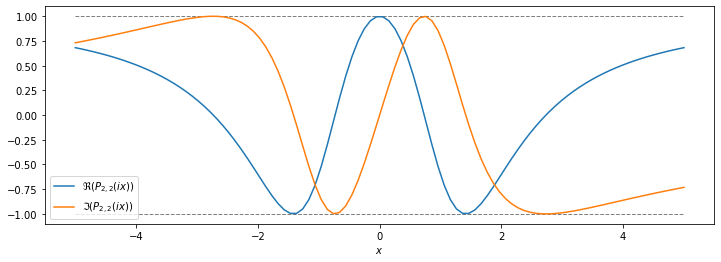
\includegraphics[height=0.35\textheight]{img/P22_reim}
   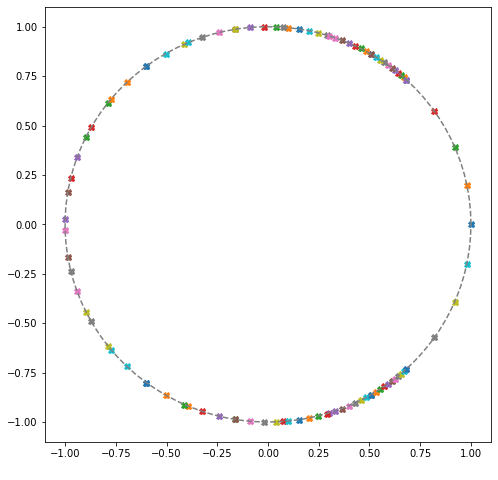
\includegraphics[height=0.35\textheight]{img/P22_ev}
   \caption{$P_{2,2}(\I x)$, $x\in[-5,5]$}
 \end{figure}
\end{frame}

\begin{frame}{Eigenvalues of assymetric Padé approximants}
  \begin{columns}
    \begin{column}{0.5\textwidth}
      \begin{figure}\centering 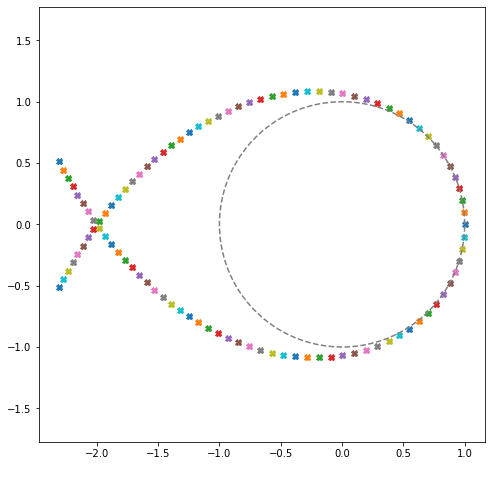
\includegraphics[width=\textwidth]{img/P21_ev} \caption{$P_{2,1}(\I x)$ $x\in[-5,5]$}\end{figure}
    \end{column}
    \begin{column}{0.5\textwidth}
      \begin{figure}\centering 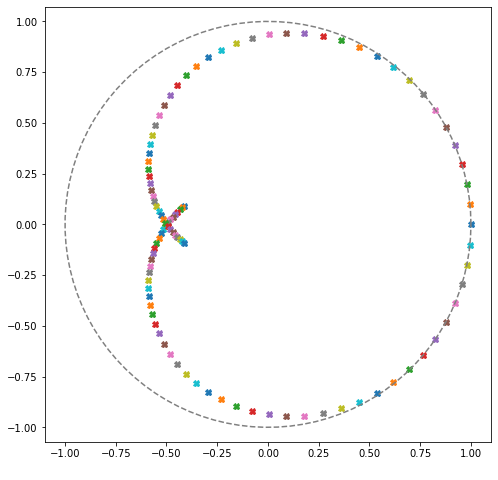
\includegraphics[width=\textwidth]{img/P12_ev} \caption{$P_{1,2}(\I x)$ $x\in[-5,5]$}\end{figure}
    \end{column}
  \end{columns}
\end{frame}

\begin{frame}{Splitting method}
  \vspace{-2cm}\hfill\begin{turn}{-30}{\mbold{\textcolor{mred}{Breaking news!}}}\end{turn}

  We can also approximate $e^{\tau L}$ with troncature of BCH formula or splitting method:
  $$
    L = \underbrace{\begin{pmatrix}
      \gz & \hspace{-0.25cm}-B_0 & \gz                   & \gz                   & \hspace{-0.125cm}\Omega_{pe}^2\hspace{-0.125cm} &                  \gz                            & \gz \\ 
      B_0 &                  \gz & \gz                   & \gz                   &                  \gz                            & \hspace{-0.125cm}\Omega_{pe}^2\hspace{-0.125cm} & \gz \\
      \gz &                  \gz & \gz                   & \gz                   &                  \gz                            &                  \textcolor{violet}{0}          & \gz \\ 
      \gz &                  \gz & \gz                   & \gz                   &                  \textcolor{violet}{0}          &                  \gz                            & \gz \\ 
      -1  &                  \gz & \gz                   & \textcolor{violet}{0} &                  \gz                            &                  \gz                            & \gz \\ 
      \gz & \hspace{-0.25cm}-1   & \textcolor{violet}{0} & \gz                   &                  \gz                            &                  \gz                            & \gz \\ 
      \gz &                  \gz & \gz                   & \gz                   &                  \gz                            &                  \gz                            & \hspace{-0.25cm}-\I v_z\kappa \\ 
    \end{pmatrix}}_{L_1}
    +
    \underbrace{\begin{pmatrix}
      \gz & \textcolor{violet}{0} & \gz                      &  \gz                      &  \textcolor{violet}{0}            & \gz                      & \gz \\ 
      \textcolor{violet}{0} &  \gz & \gz                      &  \gz                      &  \gz                      & \textcolor{violet}{0}            & \gz \\
      \gz &  \gz & \gz                      &  \gz                      &  \gz                      & \hspace{-0.125cm}{\I\kappa}\hspace{-0.125cm} & \gz \\ 
      \gz &  \gz & \gz                      &  \gz                      & \hspace{-0.125cm}{-\I\kappa}\hspace{-0.125cm} & \gz                      & \gz \\ 
      \textcolor{violet}{0}  &  \gz & \gz                      & \hspace{-0.125cm}{-\I\kappa}\hspace{-0.125cm} &  \gz                      & \gz                      & \gz \\ 
      \gz & \textcolor{violet}{0}   & \hspace{-0.125cm}{\I\kappa}\hspace{-0.125cm} &  \gz                      &  \gz                      & \gz                      & \gz \\ 
      \gz &  \gz & \gz                      &  \gz                      &  \gz                      & \gz                      & \textcolor{violet}{0} \\ 
    \end{pmatrix}}_{L_2}
  $$
  $$
    e^{\tau L} \approx e^{\frac{\tau}{2}L_1}e^{\tau L_2}e^{\frac{\tau}{2}L_1} = S_{\tau}(L)
  $$
\end{frame}

%\newcommand{\pexp}[1]{\textcolor{violet}{P_{\!\!p,q}\!\left(#1\right)}}
\newcommand{\pexp}[1]{\textcolor{violet}{ \epsilon^{#1} }}
\begin{frame}{Error on approximate Lawson method}
  We note $P_{p,q}(z) = \pexp{z}$.
  We recall: $$\pexp{\tau L} = e^{\tau L} + \mathcal{O}(\tau^{r+1}),\quad\text{with}\ r=p+q$$

  Lawson RK(3,3) method becomes:
  $$
    \begin{aligned}
      \!\!\!\!u^{(1)} &= \pexp{\Delta t L}u^n + \Delta t\pexp{\Delta t L}N(t^n,u^n) \\
      \!\!\!\!u^{(2)} &= \frac{3}{4}\pexp{\!\frac{\Delta t}{2} L\!}u^n + \frac{1}{4}\pexp{\!\!-\frac{\Delta t}{2} L\!}u^{(1)} + \frac{\Delta t}{4}\pexp{\!\!-\frac{\Delta t}{2} L\!} N(t^n+\Delta t,u^{(1)}) \\
      \!\!\!\!u^{n+1} &= \frac{1}{3}\pexp{\Delta t L}u^n + \frac{2}{3}\pexp{\!\frac{\Delta t}{2} L\!}u^{(2)} + \frac{2}{3}\Delta t \pexp{\!\frac{\Delta t}{2} L\!} N(t^n+\frac{\Delta t}{2},u^{(2)})
    \end{aligned}
  $$
  \mbold{If} $L$ and $N$ commute: $u^{n+1} = \pexp{\Delta tL}\left(I + N + \frac{N^2}{2} + \frac{N^3}{6} \right)u^n$, stability is same as RK(3,3).
  \begin{thebibliography}{9}
    \setbeamertemplate{bibliography item}[article]
    \bibitem{k} \customcite{Crouseilles:2019b} \textcolor{defaultcolor}{study of Lawson stability in scalar case}
  \end{thebibliography}
   \mbold{Else}\dots

\end{frame}
\begin{frame}{Error on approximate Lawson method}
  \mbold{If} $L$ and $N$ don't commute:
  $$
    \begin{aligned}
      u^{n+1} = \Big[ \pexp{\Delta tL}
        &+\Delta t\left(\frac{2}{3}\pexp{\frac{\Delta t}{2}L}N\pexp{\frac{\Delta t}{2}L}+\frac{1}{6}\pexp{\Delta tL}N + \frac{1}{6}N\pexp{\Delta tL}\right)
          \textcolor{gris}{\rightsquigarrow \pexp{\Delta L}\Delta t N} \\
        & + \frac{\Delta t^2}{2}\left(\frac{1}{3}N\pexp{\Delta tL}N + \frac{1}{3}\pexp{\frac{\Delta t}{2}L}N\pexp{\frac{\Delta t}{2}L}N + \frac{1}{3} \pexp{\frac{\Delta t}{2}L}N\pexp{-\frac{\Delta t}{2}L}N\pexp{\Delta tL} \right) \\
          &\hspace{2cm} \textcolor{gris}{\rightsquigarrow \pexp{\Delta L}\frac{\left(\Delta t N\right)^2}{2}} \\
      & + \frac{\Delta t^3}{6}\pexp{\frac{\Delta t}{2}L}N\pexp{-\frac{\Delta t}{2}L}N\pexp{\Delta tL}N \Big]u^n \textcolor{gris}{\rightsquigarrow \pexp{\Delta L}\frac{\left(\Delta t N\right)^3}{6}}
    \end{aligned}
  $$

  \begin{lemma}
    Trucature error of modified Lawson RK($s$,$m$) is in $\mathcal{O}(\Delta t^{\min(r,m)})$
  \end{lemma}
\end{frame}

\begin{frame}{Test 1: measure of order}
  Simulation of $\partial_t u + a\partial_x u + b\partial_y u = 0$ (2D translation test case).
  \begin{figure}
    \centering
    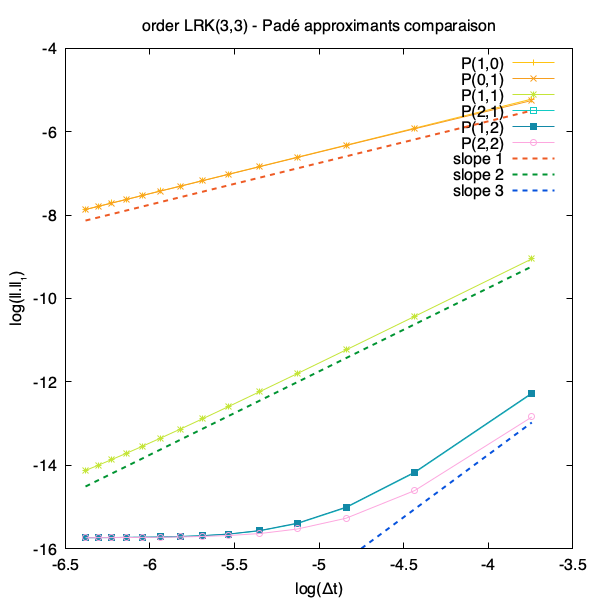
\includegraphics[height=0.6\textheight]{img/order_lrk33pade}
    \caption{Order of Lawson RK(3,3) $P(p,q)$ approximant, $p=1,2$, $q=1,2$}
  \end{figure}
\end{frame}
\begin{frame}{Test 2: illustration of instability or stability}
  Simulation of $\partial_t u - y\partial_x u + x\partial_y u = 0$ (2D rotation)
  \begin{figure}
    \centering
    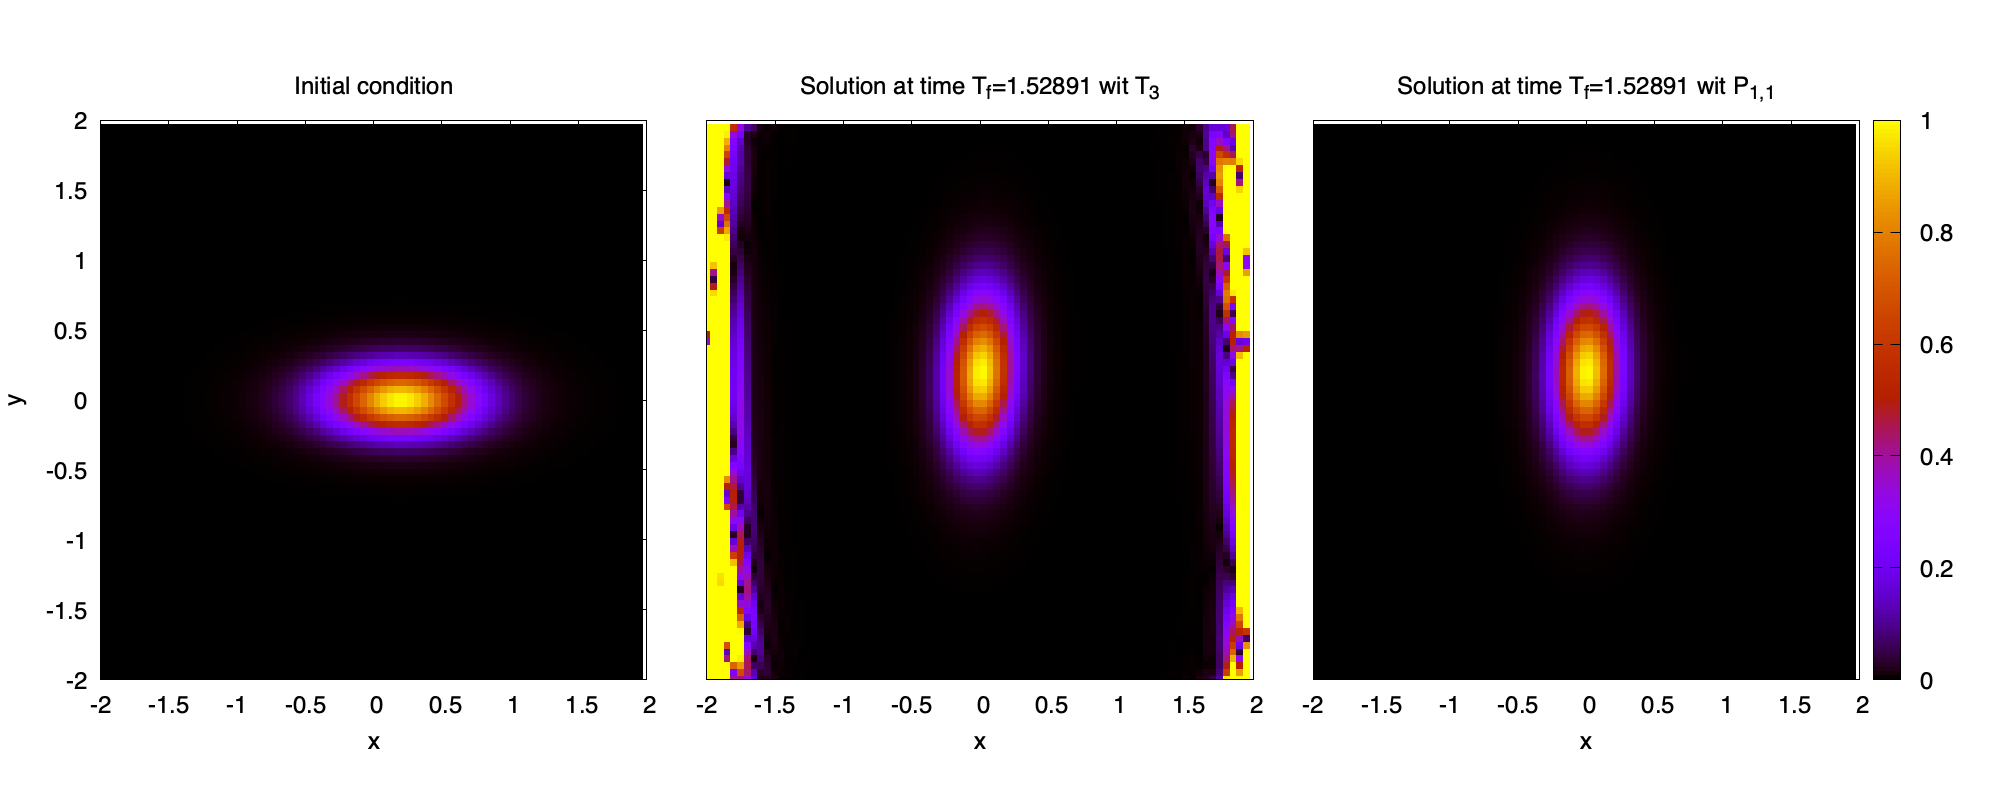
\includegraphics[width=\textwidth]{img/uf_t3p11}
    \caption{Initial condition (left), solution with Lawson RK(3,3) $T(3)$ series (middle) and Lawson RK(3,3) $P(1,1)$ approximant (right)}
  \end{figure}
\end{frame}

% -------------------------------------------------------------------
% --- NUMERICAL RESULTS ---------------------------------------------
% -------------------------------------------------------------------
\changecolor{sec4}
\section{Numerical results}
\begin{frame}{Numerical results}
  We compare:
  \begin{itemize}
    \item Splitting method:\begin{itemize}
      \item Strang (order 2)
      \item Suzuki (order 4)
    \end{itemize}
    \item Lawson method:\begin{itemize}
      \item LRK(4,4) (order 4)
      \item LDP4(3) (adaptive time step method)
    \end{itemize}
    \item Lawson method with approximation of linear part:\begin{itemize}
      \item LRK(4,4) with Padé $(2,2)$ (order 4 + approximation of order $2+2=4$)
      \item LDP4(3) with Padé $(2,2)$ (adaptive time step method)
    \end{itemize}
  \end{itemize}

  \mbold{But:} Padé approximant implies a huge rational function (with invert of matrix), high order Lawson methods have a lot of coefficients, with 7 variables problem\dots \ \arrow \ bug source !!!
\end{frame}
\begin{frame}{Code generator}
  % The main idea of code generator:
  % \begin{enumerate}
  %   \item Write with SymPy the Lawson method with a vector $U\in\mathbb{C}^7$, an abstract matrix $L\in\mathcal{M}_7(\mathbb{C})$ and an abstract nonlinear part $N:t,U\mapsto N(t,U)\in\mathbb{C}^7$
  %   \item Compute $e^{\tau L}$ with our $L$ matrix, and given approximation of $\exp$
  %   \item Loop for each stage of Lawson method into a code template (Jinja2)
  %   \item Save the file, compile and run with a given configuration file
  % \end{enumerate}
  
  \begin{figure}
    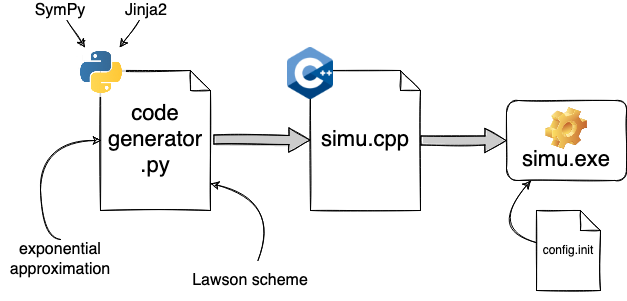
\includegraphics[width=\textwidth]{img/codegen}
  \end{figure}
\end{frame}

\begin{frame}{Numerical test}
  Weibel instability:
  $$
    \begin{cases}
      \Mvb{j}_c(t=0,z) = 0 \\
      \Mvb{B}(t=0,z) = \left( \epsilon \sin(Kz) , 0 \right) \\
      \Mvb{E}(t=0,z) = 0 \\
      f_h(t=0,z,\Mvb{v}) = \dfrac{\rho_h}{ (2\pi)^{3/2} \bar{v}_\perp^2 \bar{v}_\parallel }\exp( -\dfrac{v_z^2}{2\bar{v}_\parallel^2} - \dfrac{(v_x^2 + v_y^2)}{2\bar{v}_\perp^2}  )
    \end{cases}
  $$
  with $z\in[0,\frac{2\pi}{K}]$, $\Mvb{v}\in[-3.6,3.6]\times[-3.6,3.6]\times[-2.4,2.4]$, $K=2$, $\bar{v}_\parallel=0.2$, $\bar{v}_\perp = 0.6$, $\rho_h=0.2$ and $\epsilon=10^{-5}$.

  \mbold{Compare energies:}
  $$
    \mathcal{H}_E(t) = \frac{1}{2}\int {\| \Mvb{E}(t,z) \|_2}^2\dd{z}
    \qquad
    \mathcal{H}_B(t) = \frac{1}{2}\int {\| \Mvb{B}(t,z) \|_2}^2\dd{z}
  $$
  $$
    \mathcal{H}_c(t) = \frac{1}{2\Omega_{pe}^2}\int {\| \Mvb{j}_c(t,z) \|_2}^2\dd{z}
  $$
\end{frame}

\begin{frame}{Numerical results: splitting vs Lawson}
  {$N_z\times N_{v_x} \times N_{v_y} \times N_{v_z} = 27 \times 32 \times 32 \times 41$}
  \only<1>{
    \begin{figure}
      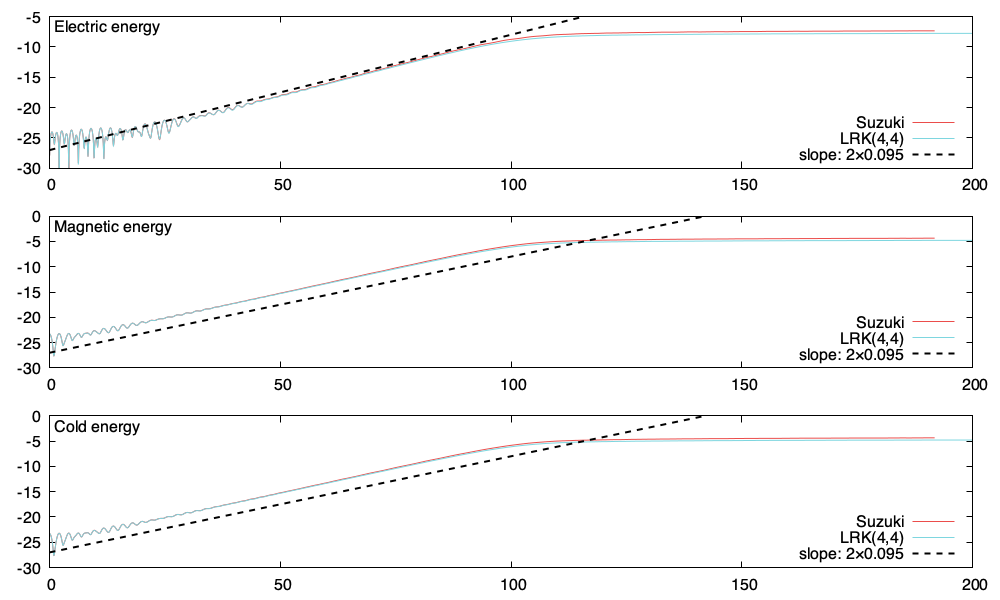
\includegraphics[height=0.75\textheight]{img/energy_slrkp}
      \vspace{-0.25cm}
      \caption{Energies evolution, $\Delta t = 0.05$}
    \end{figure}
  }
  \only<2>{
    \begin{figure}
      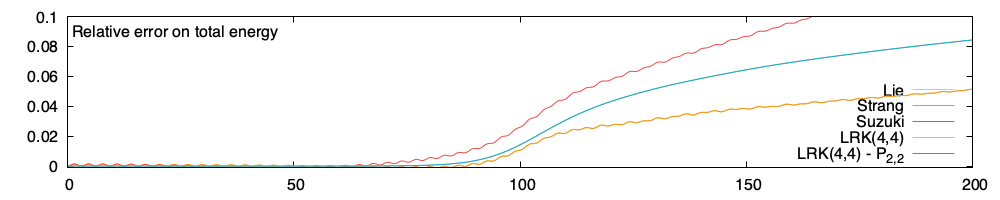
\includegraphics[width=\textwidth]{img/error_slrkp}
      \caption{Relative error on total energy, $\Delta t = 0.05$}
    \end{figure}
  }
  \only<3>{
    \begin{table}[h]
      \centering
      \begin{tabular}{l|r}
        time integrator & simulation time \\
        \hline
        Lie splitting        &                $13\,\text{h}\ 25\,\text{min}\ 10\,\text{s}$ \\
        Strang splitting     &                $17\,\text{h}\ 09\,\text{min}\ 54\,\text{s}$ \\
        Suzuki splitting     &   $3\,\text{j}\ 03\,\text{h}\ 05\,\text{min}\ 24\,\text{s}$ \\
        \hline
        LRK(3,3)             &                $11\,\text{h}\ 29\,\text{min}\ 09\,\text{s}$ \\
        \hline
        LRK(4,4)             &                $14\,\text{h}\ 06\,\text{min}\ 15\,\text{s}$ \\
      \end{tabular}
      \caption{Simulation time for some simulation, on mesh $N_z \times N_{v_x} \times N_{v_y} \times N_{v_z}=27\times32\times32\times41$ and time step $\Delta t = 0.05$.}
    \end{table}
  }
\end{frame}

\begin{frame}{Numerical results: Padé-Lawson}
  \begin{figure}
    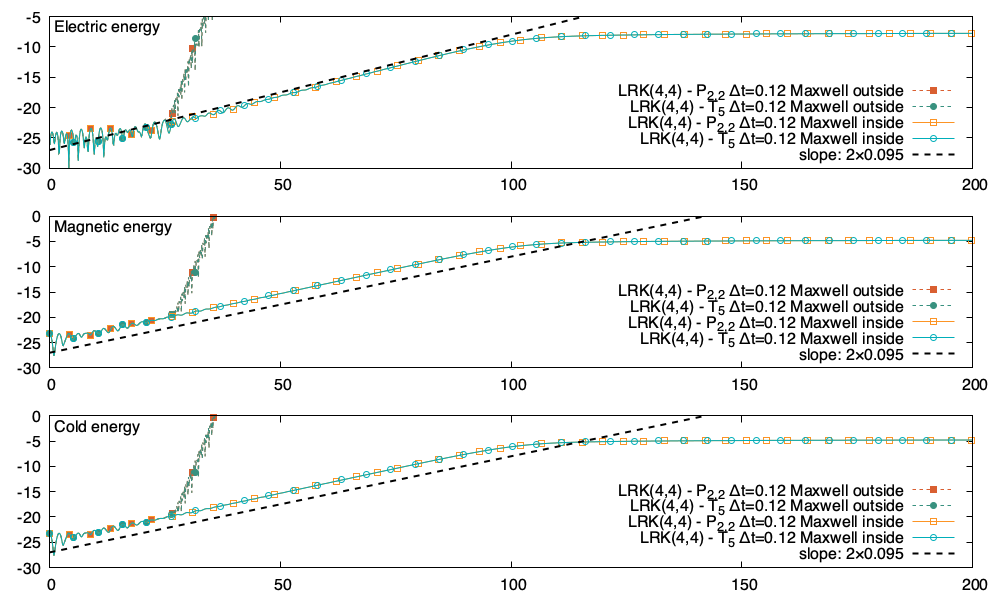
\includegraphics[height=0.75\textheight]{img/energy_lrkpt_m}
    \vspace{-0.25cm}
    \caption{Energies evolution, Lawson with Taylor or Padé approximation, $\Delta t = 0.12$}
  \end{figure}
\end{frame}
\begin{frame}{Numerical results: Padé-Lawson adaptive time step}
  \only<1>{
    \begin{figure}
      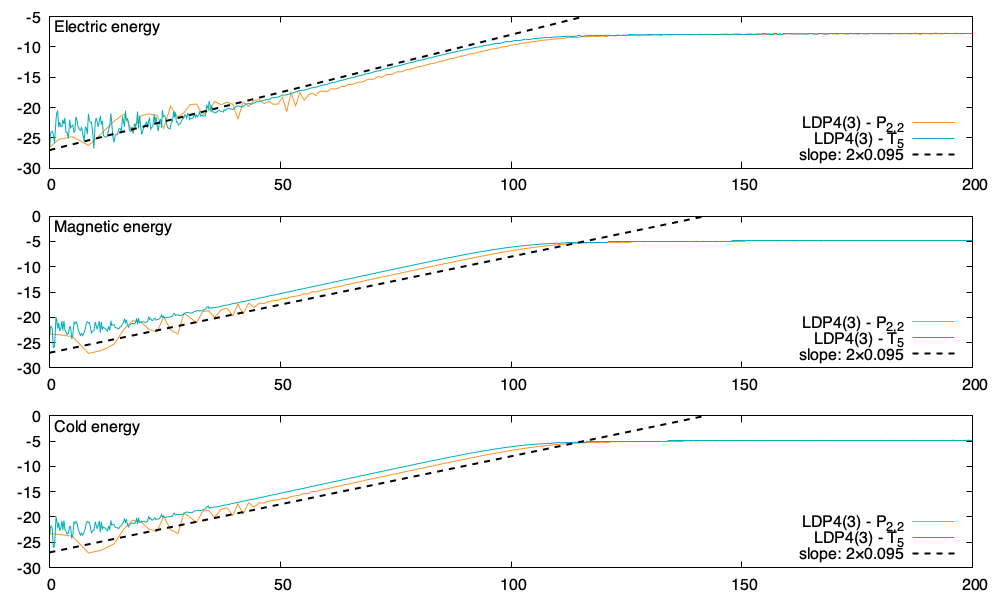
\includegraphics[height=0.72\textheight]{img/energy_ldppt}
      \vspace{-0.25cm}
      \caption{Energies evolution, Lawson with Taylor or Padé approximation, $\Delta t^n$}
    \end{figure}
  }
  \only<2>{
    \begin{figure}
      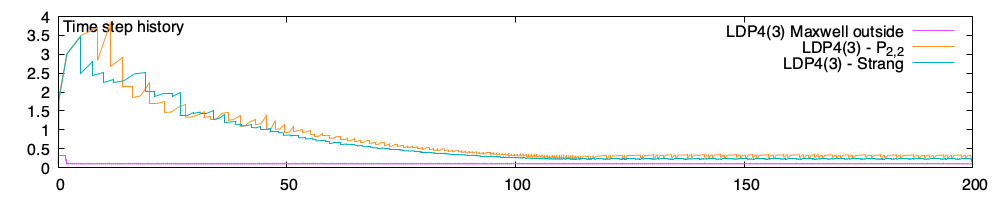
\includegraphics[width=\textwidth]{img/dt_ldppt}
      \caption{Time step evolution and estimate of local error, Lawson with Taylor or Padé approximation, $\Delta t^n$}
    \end{figure}
  }
\end{frame}
  \begin{frame}{Simulation time}
  \begin{table}[h]
    \centering
    \begin{tabular}{l|r}
      time integrator & simulation time \\
      \hline
      LRK(3,3)             &                $11\,\text{h}\ 29\,\text{min}\ 09\,\text{s}$ \\
      LRK(3,3) - $P_{1,1}$ &                $10\,\text{h}\ 54\,\text{min}\ 11\,\text{s}$ \\
      LRK(3,3) - $P_{2,2}$ &                $10\,\text{h}\ 55\,\text{min}\ 26\,\text{s}$ \\
      \hline
      LRK(4,4)             &                $14\,\text{h}\ 06\,\text{min}\ 15\,\text{s}$ \\
      LRK(4,4) - $P_{2,2}$ &                $13\,\text{h}\ 59\,\text{min}\ 59\,\text{s}$ \\
      \hline
      LDP4(3)              &                $11\,\text{h}\ 44\,\text{min}\ 04\,\text{s}$ \\
      LDP4(3) - $P_{2,2}$  &                $04\,\text{h}\ 09\,\text{min}\ 44\,\text{s}$ \\
    \end{tabular}
    \caption{Simulation time for some simulation, on mesh $N_z \times N_{v_x} \times N_{v_y} \times N_{v_z}=27\times32\times32\times41$ and time step $\Delta t = 0.05$ (initial time step for adaptive time step strategy).}
  \end{table}
\end{frame}

% -------------------------------------------------------------------
% --- CONCLUSION ----------------------------------------------------
% -------------------------------------------------------------------
\changecolor{sec5}
\section{Conclusion}
\begin{frame}{Conclusion}
  \begin{enumerate}
    \item[\cmark] First simulations of this system using Hamiltonian splitting
    \item[\xmark] Numerical cost of splitting methods (not bad in $1dz-1dv$ but very bad in $1dz-3dv$, must be very very very bad in $3dx-3dv$)
    \item[\cmark] Numerical cost of Lawson methods
    \item[\bmark] Behavior of total energy of Lawson method (but we can use high order method easily)
    \item[\cmark] Error of approximation with Padé approximant can be lower than time integrator
  \end{enumerate}
\end{frame}
\begin{frame}{Future works}
  \begin{itemize}
    \item Compare Lawson method with Padé approximant with a PIC simulation
    \item Add $\int \Mvb{v}f_h\dd{\Mvb{v}}$ in linear part (for $1dx-1dv$ model)
  \end{itemize}
\end{frame}

% -------------------------------------------------------------------
% --- THANKS --------------------------------------------------------
% -------------------------------------------------------------------

\changecolor{PLB}
\begin{frame}[t]
  \vfill
  {\usebeamerfont{title} Thank you for your attention}
  \vfill
\end{frame}
\appendix
\backupbegin

% -------------------------------------------------------------------
% --- BACKUP --------------------------------------------------------
% -------------------------------------------------------------------
\begin{frame}[plain]
  \vspace{0.65\textwidth}
  \hfill\footnotesize{Backup}
\end{frame}
% -------------------------------------------------------------------
\begin{bframe}{Adaptive time step method for splitting method}
  \begin{thebibliography}{9}
    \setbeamertemplate{bibliography item}[article]
    \bibitem{backup:a} \customcite{Blanes:2019} \textcolor{defaultcolor}{for Suzuki splitting method}
  \end{thebibliography}
  $$
    u^{n+1}_{[4]} = \mathcal{S}_{\Delta t}(u^n)
      = S_{\alpha_1\Delta t}
        \circ \underbrace{ S_{\alpha_2\Delta t}
        \circ \underbrace{ S_{\alpha_3\Delta t}
        \circ \underbrace{ S_{\alpha_2\Delta t}
        \circ \underbrace{ S_{\alpha_1\Delta t} (u^n). }_{u^{(1)}}
                                                       }_{u^{(2)}}
                                                       }_{u^{(3)}}
                                                       }_{u^{(4)}}
  $$
  We compute an order 3 approximation from $U^n$ and $U^{(s)}$, $s=1,2,3,4$ :
  $$
    u^{n+1}_{[3]} = -u^n + w_1(u^{(1)}+u^{(4)}) + w_2(u^{(2)}+u^{(3)})
  $$
  with:
  $$
    w_1 = \frac{g_2(1-g_2)}{g_1(g_1-1)-g_2(g_2-1)},\quad w_2 = 1-w_1, \quad \begin{aligned}g_1 &= \alpha_1\\ g_2&=\alpha_1+\alpha_2\end{aligned}
  $$
  and $L^{n}_{[3]} = \left\| u^{n+1}_{[4]} - u^{n+1}_{[3]} \right\|_2$
\end{bframe}
%-------%
\begin{bframe}{Adaptive time step method for Lawson method}
  Lawson methods are built on Runge-Kutta method, embedded Lawson method are written with an underlying embedded Runge-Kutta method.

  \begin{thebibliography}{9}
    \setbeamertemplate{bibliography item}[article]
    \bibitem{backup:b} \customcite{Dormand:1978}
  \end{thebibliography}
  With DP4(3) (Dormand-Prince method of order 4, with embedded 3 method):
    $$
    \begin{array}{c|cccccc}
      0           &             &             &             &             &                & \multirow{5}{*}{$\left.\phantom{\begin{matrix}0\\1\\2\\3\\4\end{matrix}}\right\}$Classical RK(4,4)} \\
      \frac{1}{2} & \frac{1}{2} &             &             &             &                & \\
      \frac{1}{2} & 0           & \frac{1}{2} &             &             &                & \\
      1           & 0           & 0           & 1           &             &                & \\
    \cline{1-6}
      1           & \frac{1}{6} & \frac{1}{3} & \frac{1}{3} & \frac{1}{6} &                &\\
    \cline{1-6}
                  & \frac{1}{6} & \frac{1}{3} & \frac{1}{3} & \frac{2}{30} & \frac{1}{10}  & 
    \end{array}
  $$
  We compute a 3\textsuperscript{rd} order approximation from $u^n$, $u^{(s)}$, $s=1,2,3,4$ done by the last line of Butcher tableau.

  And $L^{n}_{[3]} = \left\| u^{n+1}_{[4]} - u^{n+1}_{[3]} \right\|_2$
\end{bframe}
% -------------------------------------------------------------------
\begin{bframe}{Poisson bracket}
  For two given functionals  $\mathcal{F}$, $\mathcal{G}$ of $\Mvb{j}_c$, $\Mvb{B}$, $\Mvb{E}$, $f_h$, the Poisson bracket is given by 
  $$
    \begin{aligned}
      \{ {\cal F}, {\cal G} \}[\Mvb{j}_c, \Mvb{B}, \Mvb{E}, f_h] &=
          \frac{1}{m_e} \int_\Omega \int_{\mathbb{R}^3} f_h \Big[ \frac{\delta \mathcal{F}}{\delta f_h}, \frac{\delta \mathcal{G}}{\delta f_h} \Big]_{\Mvb{x}\Mvb{v}} \dd{\Mvb{v}}\dd{\Mvb{x}} \\
      & + \frac{q_e}{m_e\varepsilon_0} \int_\Omega \int_{\mathbb{R}^3} f_h \left( \nabla_{\Mvb{v}}\frac{\delta \mathcal{F}}{\delta f_h} \cdot \frac{\delta \mathcal{G}}{\delta\Mvb{E}} -  \nabla_{\Mvb{v}}\frac{\delta \mathcal{G}}{\delta f_h} \cdot \frac{\delta \mathcal{F}}{\delta\Mvb{E}} \right) \dd{\Mvb{v}}\dd{\Mvb{x}} \\
      & + \frac{q_e}{m^2_e} \int_\Omega \int_{\mathbb{R}^3} f_h (\Mvb{B} + \Mvb{B}_0) \cdot \left( \nabla_{\Mvb{v}}\frac{\delta \mathcal{F}}{\delta f_h} \times \nabla_{\Mvb{v}}\frac{\delta \mathcal{G}}{\delta f_h} \right) \dd{\Mvb{v}}\dd{\Mvb{x}} \\
      & + \frac{1}{\varepsilon_0} \int_\Omega  \left( \nabla \times \frac{\delta \mathcal{F}}{\delta \Mvb{E}} \cdot  \frac{\delta \mathcal{G}}{\delta \Mvb{B}} - \nabla \times \frac{\delta \mathcal{G}}{\delta \Mvb{E}} \cdot  \frac{\delta \mathcal{F}}{\delta \Mvb{B}} \right) \dd{\Mvb{x}} \\
      & +  \int_\Omega \Omega_{pe}^2 \left( \frac{\delta \mathcal{F}}{\delta \Mvb{j}_c} \cdot \frac{\delta \mathcal{G}}{\delta \Mvb{E}} -  \frac{\delta \mathcal{G}}{\delta \Mvb{j}_c} \cdot \frac{\delta \mathcal{F}}{\delta \Mvb{E}} \right)  \dd{\Mvb{x}} \\
      & + \frac{q_e \varepsilon_0}{m_e}  \int_\Omega   \Omega_{pe}^2 \Mvb{B}_0 \cdot \left( \frac{\delta \mathcal{F}}{\delta \Mvb{j}_c} \times \frac{\delta \mathcal{G}}{\delta \Mvb{j}_c} \right) \dd{\Mvb{x}}.
    \end{aligned}
  $$
\end{bframe}
\begin{bframe}{Splitting method $\varphi^{[j_c]}$}
  $$
    \varphi^{[j_c]}(U) =
    \begin{cases}
      \partial_t \Mvb{j}_c = -J\Mvb{j}B_0 \\
      \partial_t \Mvb{B} = 0 \\
      \partial_t \Mvb{E} = -\Mvb{j}_c \\
      \partial_t f_h = 0
    \end{cases}
    \rightarrow
    \varphi_{t}^{[j_c]}(U^0) = \begin{pmatrix}
      e^{-tJ}\Mvb{j}_c(0)B_0 \\
      \Mvb{B}(0) \\
      \Mvb{E}(0) - J(e^{-tJ}-I)\Mvb{j}_c(0) \\
      f_h(0)
    \end{pmatrix}
  $$
  Obtain because: $\int_0^t \exp(-sJ)\Mvb{j}_c(0)\dd{s} = J(\exp(-tJ)-I)\Mvb{j}_c(0)$, with:
  $$
    \exp(-tJ) = \begin{pmatrix}\cos(t) & -\sin(t) \\ \sin(t) & \cos(t) \end{pmatrix}
  $$
\end{bframe}
\begin{bframe}{Splitting method $\varphi^{[B]}$}
  $$
    \varphi^{[B]}(U) =
    \begin{cases}
      \partial_t \Mvb{j}_c = 0 \\
      \partial_t \Mvb{B} = 0 \\
      \partial_t \Mvb{E} = -J\partial_z\Mvb{B} \\
      \partial_t f_h = 0
    \end{cases}
    \rightarrow
    \varphi_{t}^{[B]}(U^0) = \begin{pmatrix}
      \Mvb{j}_c(0) \\
      \Mvb{B}(0) \\
      \Mvb{E}(0) - tJ\partial_z\Mvb{B}(0) \\
      f_h(0)
    \end{pmatrix}
  $$
  \mbold{Numerical tools:}
  \begin{itemize}
    \item Solve in Fourier space
  \end{itemize}
\end{bframe}
\begin{bframe}{Splitting method $\varphi^{[E]}$}
  $$
    \varphi^{[E]}(U) =
    \begin{cases}
      \partial_t \Mvb{j}_c = \Omega_{pe}^2\Mvb{E} \\
      \partial_t \Mvb{B} = J\partial_z\Mvb{E} \\
      \partial_t \Mvb{E} = 0 \\
      \partial_t f_h = \Mvb{E}\cdot\nabla_{\Mvb{v}}f_h
    \end{cases}
    \rightarrow
    \varphi_{t}^{[E]}(U^0) = \begin{pmatrix}
      \Mvb{j}_c(0) + t\Omega_{pe}^2\Mvb{E}(0) \\
      \Mvb{B}(0) + tJ\partial_z\Mvb{E}(0) \\
      \Mvb{E}(0) \\
      f_h(0,z,\Mvb{v}+t\Mvb{E}(0),v_z)
    \end{pmatrix}
  $$
  \mbold{Numerical tools:}
  \begin{itemize}
    \item 2D interpolation with 2 Lagrange 5 interpolations to approximate $f_h(0,z,\Mvb{v}+t\Mvb{E}(0),v_z)$
  \end{itemize}
\end{bframe}
\begin{bframe}{Splitting method $\varphi^{[f_h]}$}
  $$
    \varphi^{[f_h]}(U) =
    \begin{cases}
      \partial_t \Mvb{j}_c = 0 \\
      \partial_t \Mvb{B} = 0 \\
      \partial_t \Mvb{E} = \int\Mvb{v}f_h\dd{\Mvb{v}} \\
      \partial_t f_h = -v_z\partial_zf_h + (\Mvb{v}\times(\Mvb{B}+\Mvb{B}_0))\cdot\nabla_{\Mvb{v}}f_h
    \end{cases}
  $$
  This step is split again onto 3 parts.
\end{bframe}
\begin{bframe}{Splitting method $\varphi^{[f_h]}$, $f_{h,\star}$, $\star\in\{x,y\}$}
  $$
    \!\!\varphi^{[f_{h,x}]}(U)\!=\!\!
    \begin{cases}
      \partial_t \Mvb{j}_c = 0 \\
      \partial_t \Mvb{B} = 0 \\
      \partial_t E_x = \int\!v_x f_h\dd{\Mvb{v}} \\
      \partial_t E_y = 0 \\
      \partial_t f_h = -v_x B_0\partial_{v_y} f_h + v_x B_y\partial_{v_z}f_h 
    \end{cases}
    \hspace{-2.625cm}
    \rightarrow
    \varphi_t^{[f_{h,x}]}(U^0)\!=\!\!\begin{pmatrix}
      \Mvb{j}_c(0) \\
      \Mvb{B}(0) \\
      E_x(0) + t\int\!v_xf_h(0)\dd{\Mvb{v}} \\
      E_y(0) \\
      \!f_h(\!0,\!z,\!\!v_x,\!\!v_y\!\!-\!\!tv_x\!B_0,\!v_z\!\!+\!\!tB_y\!v_x\!)\!
    \end{pmatrix}
  $$
  \mbold{Numerical tools:}
  \begin{itemize}
    \item 2D interpolation with Lagrange 5 interpolation to approximate $f_h(0,z,v_x,v_y-tv_xB_0,v_z+tB_yv_x)$
  \end{itemize}
  Same thing for $\varphi^{[f_{h,y}]}$ in $v_y$ direction.
\end{bframe}
\begin{bframe}{Splitting method $\varphi^{[f_h]}$, $f_{h,z}$}
  $$
    \varphi^{[f_{h,z}]}(U) =
    \begin{cases}
      \partial_t \Mvb{j}_c = 0 \\
      \partial_t \Mvb{B} = 0 \\
      \partial_t \Mvb{E} = 0 \\
      \partial_t f_h = -v_z\partial_zf_h + (-v_zB_y\partial_{v_x}f_h + v_zB_x\partial_{v_y}f_h) 
    \end{cases}
  $$
  \mbold{Numerical tools:}
  \begin{itemize}
    \item Split \mbold{again} onto 3 parts, with change of variable $g(t,z,\Mvb{v}):=f(t,z+tv_z,\Mvb{v})$
    \item 2D interpolation with Lagrange 5 interpolation to approximate $g(0,z,v_x-\sum_k\hat{B}_{y}(0,k)\frac{1}{ik}e^{ikz}(e^{iktv_z}-1), v_y+\sum_k\hat{B}_x(0,k)\frac{1}{ik}e^{ikz}(e^{iktv_z}-1),v_z)$
     \item Revert change of variable with Fourier transform
  \end{itemize}
\end{bframe}
\begin{bframe}{Splitting method}
  For Lie method:

  $U^{n+1} = \varphi_{\Delta t}^{[j_c]}
        \circ\varphi_{\Delta t}^{[B]}
        \circ\varphi_{\Delta t}^{[E_{v_x}]}
        \circ\varphi_{\Delta t}^{[E_{v_y}]}
        \circ\varphi_{\Delta t}^{[f_{h,x,v_x}]}
        \circ\varphi_{\Delta t}^{[f_{h,x,v_z}]}
        \circ\varphi_{\Delta t}^{[f_{h,y,v_y}]}
        \circ\varphi_{\Delta t}^{[f_{h,y,v_z}]}
        \circ\varphi_{\Delta t}^{[f_{h,z,1}]}
        \circ\varphi_{\Delta t}^{[f_{h,z,2}]}
        \circ\varphi_{\Delta t}^{[f_{h,z,3}]}
        (U^n)
   $
\end{bframe}

\begin{bframe}{Suzuki vs Lawson (adaptive time step)}
  \only<1>{
    \begin{figure}
      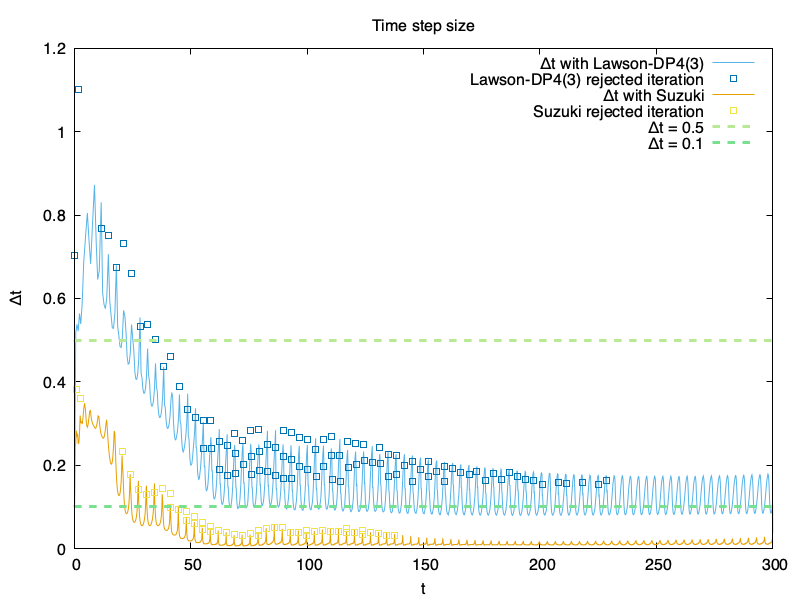
\includegraphics[height=0.8\textheight]{img/dt_size_t3}
      \caption{Time step size in 1dx-1dv}
    \end{figure}
  } \only<2>{
    \begin{figure}
      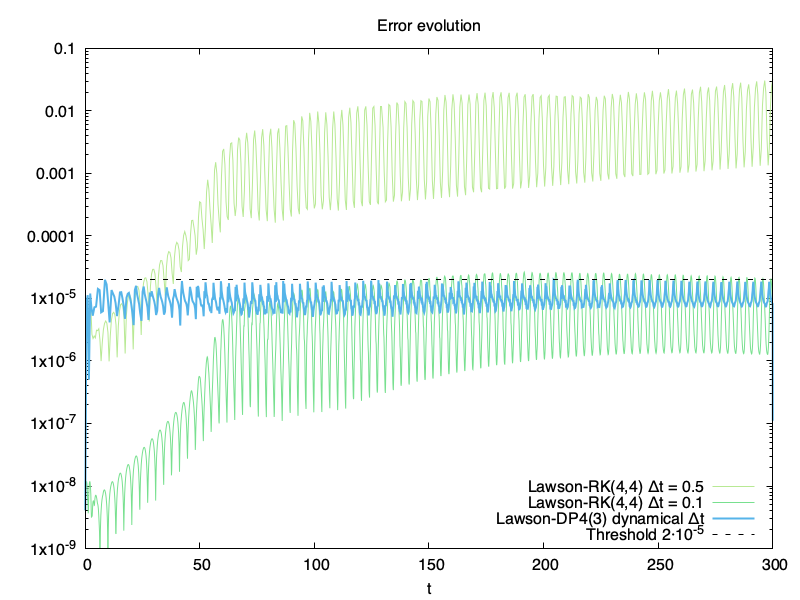
\includegraphics[width=0.48\textwidth]{img/Ll_t3}
      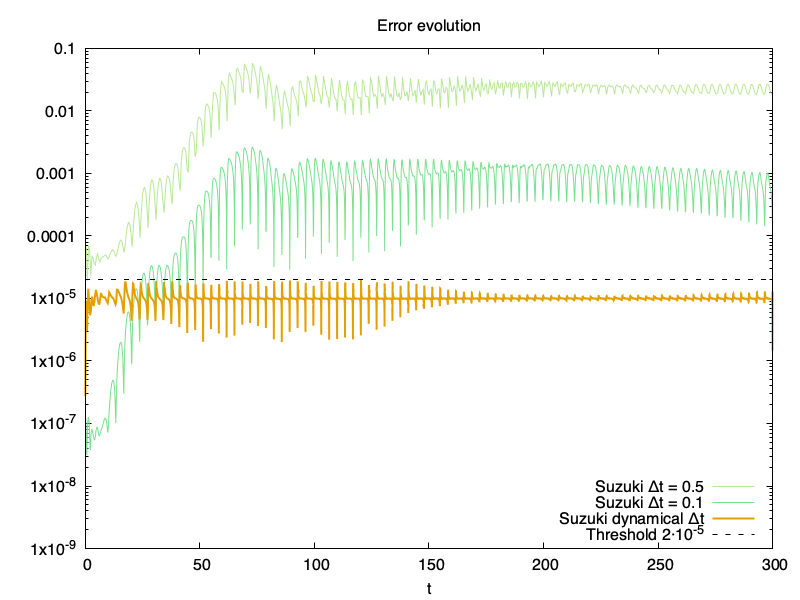
\includegraphics[width=0.48\textwidth]{img/Ls_t3}
      \caption{Local error estimate Lawson (left) and Suzuki (right)}
    \end{figure}
  }
\end{bframe}

\begin{bframe}{Time comparaison}
  \begin{figure}
    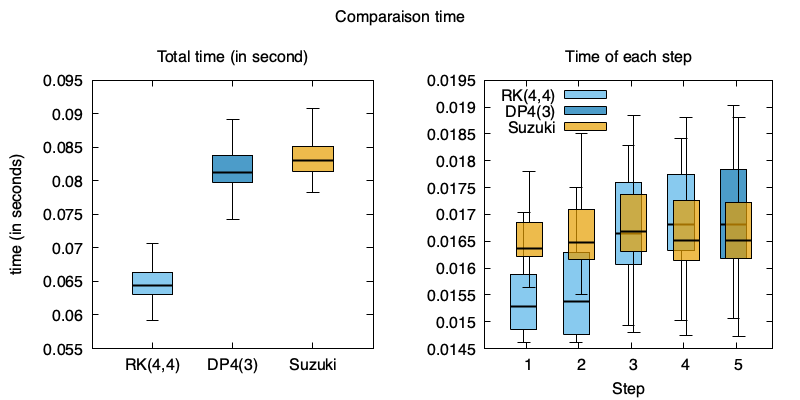
\includegraphics[width=\textwidth]{img/timer_boxplot_t4}
    \caption{Simulation time of each step}
  \end{figure}
\end{bframe}

%-------%
\backupend

\end{document}

